\chapter{Method}
\sisetup{per-mode=fraction}

This thesis implements a Generation Expansion Planning (GEP) with an energy balance approach. 

A GEP is a method to efficiently plan the investment of new generation units in a power system over a certain time horizon. It usually ends up in solving an optimization problem. A GEP optimizes the power system with new generations units taking into consideration the type, the share, the location and the time horizon of the new units. Many GEPs these days are considerably complex due to several boundary conditions such as generations types and politics, sometimes even getting non-linear \cite{GEP}. 

The GEP that is implemented in this thesis however stays linear and investment costs are not taking into consideration. This was made due to the fact that this project is in its starting phase and the first focus lies on the technical possibilities. Furthermore the time constraints of this thesis did not allow for further investigation and development of the model. 
Therefore the results obtained by this model is the needed investment in terms of MW in solar and wind and the generation dispatch over one year. 

The model was implemented in MATLAB, using the YALMIP toolbox and the Gurobi solver. 

The time horizon considered in the model is one year and the granularity is 15\,min. 

The following section elaborates the mathematical formulations for the optimization problem. 

\section{Load}
The load $P^{load}_{t}$ is a fix, inelastic parameter describing the load consumption at time $t$.

\section{Hydro Power}

\subsection{Basic Relations}
For any hydro power plant, the power at which energy is generated can be expressed by the following formula \cite{hydropower}: 

\begin{equation}\label{eq:hydro power output}
    P^{\text{out}} = \eta^{\text{t}} \cdot \rho \cdot g \cdot h \cdot Q^{\text{out}}
\end{equation}

\noindent where $P^{\text{out}}$ is the power at which energy is generated in $[\si{\W}]$, 
$\eta^{\text{t}}$ is the hydro turbine efficiency in $[\%]$ and $\rho$ is the density of water in $[\si{\kg\per\cubic\metre}]$. $g$ stands for the acceleration due to gravity in $[\si{\metre\per\square\second}]$ and $h$ symbolizes the head (i.e. the height of the waterfall) in $[\si{\metre}]$. $Q^{\text{out}}$ is the outflow rate due to generation in $[\si{\cubic\metre\per\second}]$.

The power at which water is pumped into a water reservoir can accordingly be calculated as: 

\begin{equation}\label{eq:hydro power input}
    P^{\text{in}} = \eta^{\text{p}} \cdot \rho^{\text{water}} \cdot g \cdot h \cdot Q^{\text{in,pumped}}
\end{equation}

\noindent where $P^{\text{in}}$ indicates the power at which water is pumped into the reservoir in $[\si{\W}]$, while $\eta^{\text{p}}$ is the hydro pump efficiency in $[\%]$ and $Q^{\text{in,pumped}}$ stands for the inflow rate due to pumping in $[\si{\cubic\metre\per\second}]$. The superscript "pumped" is used to avoid confusion with the natural inflow, which is denoted as $Q^{\text{in,nat}}$.

In the model no ramp up and ramp down times to reach a certain power were considered. This was made due to the fact, that with the given ramp up and down times all installed power could be reached within 15 minutes, and this is the considered granularity of the model. 

\subsection{Constraints for Run of River Power Plants}
The set of run of river power plants is denoted as $\textbf{R}$. The power output of the run of river unit $r \in \textbf{R}$ at time $t$ is denoted as $P_{r, t}$ and according to Eq.~\eqref{eq:hydro power output} defined as:

\begin{equation}\label{const:ror power output}
    P_{r, t} = \eta^{\text{t}} \cdot \rho \cdot g \cdot h_{r} \cdot Q^{\text{in,nat}}_{r, t}
\end{equation}

\noindent where $h_{r}$ denotes the head of run of river unit $r$ and $Q^{\text{in,nat}}_{r, t}$ is the natural inflow into unit $r$ at time $t$. Note that that the outflow rate due to generation ($Q^{\text{out}}$ in Eq.~\eqref{eq:hydro power output}) is assumed to be equal to the natural inflow at that time $Q^{\text{in,nat}}_{r, t}$. This is not the case in reality, but it is however a good approximation since run of river power plants cannot maintain big backwater.

Furthermore, if constraint~\eqref{const:ror power output} results in a $ P_{r, t} > P^{\text{max}}_{r}$, where $P^{\text{max}}_{r}$ denotes the installed power of unit $r$, then $ P_{r, t}$ was set equal to $P^{\text{max}}_{r}$ for this time slot.

For the simulations, the power output $ P_{r, t}$ of each unit $r$ at every time step $t$ was calculated separately and eventually summed up as $ P_{R, t} = \sum_{r \in \textbf{R}} P_{r, t}$. $ P_{R, t}$ represents the power output of all run of river power plants together. 



\subsection{Constraints for Hydro Dam Power Plants}
The set of hydro dam power plants is denoted as $\textbf{D}$. The power output and the volume of the lake of the hydro dam unit $d \in \textbf{D}$ at time $t$ are denoted as $P_{d, t}$ and $V_{d, t}$. For hydro dam power plants the following conditions are valid: 

\setlength{\belowdisplayskip}{0pt} 
\setlength{\abovedisplayskip}{0pt} 

\begin{equation}\label{const:dam boundary power}
    0 \leq P_{d, t} \leq P^{\text{max}}_{d}
\end{equation}

\begin{equation}\label{const:dam boundary volume}
    V^{\text{min}}_{d} \leq V_{d, t} \leq V^{\text{max}}_{d}
\end{equation}

\begin{equation}\label{const:dam volume start}
    V_{d, 0} = k \cdot V^{\text{max}}_{d},  \,\,\,\,\,\,\,\,\,\,     k \in [0..1]
\end{equation}

\begin{equation}\label{const:dam volume start = end}
    V_{d, 0} = V_{d, T}
\end{equation}

\setlength{\belowdisplayskip}{12pt}
\begin{equation}\label{const:dam volume update}
    V_{d, t} = V_{d, t-1} + Q^{\text{in,nat}}_{d,t} \cdot \triangle t 
    - \underbrace{\frac{P_{d, t}}{\eta^{\text{t}} g \rho h_d}}_{Q^{\text{out}}_{d,t}} \triangle t
\end{equation}

\noindent Constraint~\eqref{const:dam boundary power} limits the minimum and maximum power output of unit $d$. $P^{\text{max}}_{d}$ denotes the maximal possible output power of plant $d$. 

\noindent The water volume of the lake of unit $d$ is limited by constraint~\eqref{const:dam boundary volume}, where $V^{\text{min}}_{d}$ and $V^{\text{max}}_{d}$ indicate the lower and upper water level boundary for each lake individually. Constraint~\eqref{const:dam volume start}  defines the initial water level of each lake at the beginning of the year with reference to the maximum level. The initial volume of each lake is set equal to its end volume with constraint~\eqref{const:dam volume start = end}. 

\noindent The change in water volume during one time step $\triangle t$ is defined by constraint~\eqref{const:dam volume update}. $Q^{\text{in,nat}}_{d,t}$ is the natural inflow into the lake of plant $d$ at time $t$ and the outflow due to generation $Q^{\text{out}}_{d,t}$ is defined by Eq.~\eqref{eq:hydro power output}. 




\subsection{Constraints for Hydro Pump Power Plants}
The set of hydro pump power plants is denoted as $\textbf{P}$. They can be modelled as a storage. The discharge power (meaning power at which energy is generated) and the charge power (meaning the power at which water is pumped) of the hydro pump unit $p \in \textbf{P}$ at time $t$ are denoted as $P^{\text{dis}}_{p, t}$ and $P^{\text{cha}}_{p, t}$. The water volume of the lake of unit $p$ at time $t$ is indicated as $V_{p, t}$. For hydro pump power plants the following conditions are valid: 

\setlength{\belowdisplayskip}{0pt} 
\setlength{\abovedisplayskip}{0pt} 

\begin{equation}\label{const:pump boundary discharge power}
    0 \leq P^{\text{dis}}_{p, t} \leq B_p \cdot P^{\text{dis,max}}_{p}
\end{equation}

\begin{equation}\label{const:pump boundary charge power}
    0 \leq P^{\text{cha}}_{p, t} \leq (1-B_p) \cdot P^{\text{cha,max}}_{p}
\end{equation}

\begin{equation}\label{const:pump boundary volume}
    V^{\text{min}}_{p} \leq V_{p, t} \leq V^{\text{max}}_{p}
\end{equation}

\begin{equation}\label{const:pump volume start}
    V_{p, 0} = k \cdot V^{\text{max}}_{p},  \,\,\,\,\,\,\,\,\,\,     k \in [0..1]
\end{equation}

\begin{equation}\label{const:pump volume start = end}
    V_{p, 0} = V_{p, T}
\end{equation}

\setlength{\belowdisplayskip}{12pt}
\begin{equation}\label{const:pump volume update}
    V_{p, t} = V_{p, t-1} 
    + Q^{\text{in,nat}}_{p,t} \cdot \triangle t 
    + \underbrace{\frac{\eta^{\text{p}} P^{\text{cha}}_{p, t}}{g \rho h_p}}_{Q^{\text{in,pumped}}_{p,t}} \triangle t
    - \underbrace{\frac{P^{\text{dis}}_{p, t}}{\eta^{\text{t}} g \rho h_p}}_{Q^{\text{out}}_{p,t}} \triangle t
\end{equation}

\noindent Constraints~\eqref{const:pump boundary discharge power} and~\eqref{const:pump boundary charge power} limit the minimum and maximum discharge power and charge power. $B_p \in \{0,1\}$ denotes a binary variable guaranteeing that plant $p$ is either charging or discharging at one point in time. $P^{\text{dis,max}}_{p}$ and $P^{\text{cha,max}}_{p}$ denote the maximal possible discharging and charging power of plant $p$.

\noindent The water volume of the lake of unit $p$ is limited by constraint~\eqref{const:pump boundary volume}, where $V^{\text{min}}_{p}$ and $V^{\text{max}}_{p}$ indicate the lower and upper water level boundary for each lake individually. Constraint~\eqref{const:pump volume start}  defines the initial water level of each lake at the beginning of the year with reference to the maximum level. The initial volume of each lake is set equal to its end volume with constraint~\eqref{const:pump volume start = end}. 

\noindent The change in water volume during one time steps $\triangle t$ is defined by constraint~\eqref{const:pump volume update}. $Q^{\text{in,nat}}_{p,t}$ is the natural inflow into the lake of plant $p$ at time $t$. The the inflow $Q^{\text{in,pump}}_{p,t}$ due to charging and outflow $Q^{\text{out}}_{p,t}$ due to discharging are defined by Eq.~\eqref{eq:hydro power input} and~\eqref{eq:hydro power output} respectively. 


\section{Exchange with 50\,Hz grid}
As mentioned in the introduction, SBB operates a separate power grid at 16.7\,Hz. They own several frequency converters to exchange energy with the 50\,Hz grid. In the following the constraints for this exchange are defined. 

\subsection{Aggregation of frequency converters}
The set of frequency converters is denoted as $\textbf{F}$. Due to computational restrictions all frequency converters $f \in \textbf{F}$ where aggregated to one hypothetical frequency converter $\tilde{f}$. There exist two types of frequency converters: the static and the rotating. Since the losses are different for each type of converter, the aggregated loss $l_{\tilde{f}}$ for the hypothetical frequency converter $\tilde{f}$ is calculated as: 

\begin{equation*}
    l_{\tilde{f}} = \frac{1}{\sum_{f \in \textbf{F}} P^{\text{imp,max}}_{f}} \cdot \sum_{f \in \textbf{F}} P^{\text{imp,max}}_{f} l_{f}
\end{equation*}

\noindent where $l_{f}$ denotes the loss of converter $f$. This way the loss of each converter $f$ is weighted with its maximal import power $P^{\text{imp,max}}_{f}$.

\subsection{Constraints for the Exchange}
The power imported from the 50\,Hz to the 16.7\,Hz grid at time $t$ is $P^\text{imp}_{t}$. The power exported from the 16.7\,Hz to the 50\,Hz grid is $P^\text{exp}_{t}$. For the exchange the following constraints are valid:
 
\setlength{\belowdisplayskip}{0pt} 
\setlength{\abovedisplayskip}{0pt} 

\begin{equation}\label{const:export boundary}
    0 \leq P^{\text{imp}}_{t} \leq B_{\tilde{f}} \cdot \sum_{f \in \textbf{F}} P^{\text{imp,max}}_{f}
\end{equation}

\setlength{\belowdisplayskip}{12pt} 

\begin{equation}\label{const:import boundary}
    0 \leq P^{\text{exp}}_{t} \leq (1-B_{\tilde{f}}) \cdot \sum_{f \in \textbf{F}} P^{\text{exp,max}}_{f}
\end{equation}

\noindent where $P^{\text{imp,max}}_{f}$ and $P^{\text{exp,max}}_{f}$ are the maximum export and import power of each individual frequency transformer $f$. $B_{\tilde{f}} \in \{0,1\}$ denotes a binary variable guaranteeing that it is either exported or imported at one point in time. 

\subsection{Cost for the Exchange}
In general, no investment or operation costs were considered in the model. However the exchange with the 50\,Hz grid is not only limited by the installed powers of the frequency converters, but also by the prices. In order to limit the exchange and to introduce a seasonal pattern to the model a cost penalty for the exchange $C^{Ex}$ was introduced, which is defined as follows: 

\begin{equation}\label{const:cost}
    C^{Ex} =  C_\text{E,imp} + C_\text{P,imp} - R_\text{E,exp}
\end{equation}

\noindent where  $C_\text{E,imp}$ denotes the cost for imported energy, $C_\text{P,imp}$ denotes the cost for imported power and $R_\text{E,exp}$ indicates the revenue from exported energy. They are defined as follows:

\begin{equation}\label{const:cost import energy}
    C_\text{E,imp} = E^{\text{imp}}_{\triangle t} \cdot (KEV + AT + SDL + SP)
\end{equation}

\begin{equation}\label{const:cost import power}
    C_\text{P,imp} = LP \cdot \sum_{m \in \textbf{M}} P^\text{imp,max}_{m} 
\end{equation}

\begin{equation}\label{const:revenue export energy}
    R_\text{E,exp} = E^{\text{exp}}_{\triangle t} \cdot (1-l_{\tilde{f}}) \cdot SP
\end{equation}

\noindent In Eq.~\eqref{const:cost import energy} the imported energy $E^{\text{imp}}_{\triangle t}$ over a time step $\triangle t$ is priced with the 'Kostendeckende Einspeisevergütung' (cost-covering feed-in tariff) $KEV$, the 'Arbeitstarif' (working tariff for grid usage) $AT$, the 'Systemdienstleistungen' (system service tariff) $SDL$ and the spot price $SP$. 

\noindent The power price in Eq.~\eqref{const:cost import power} is calculated as the sum of the maximum power imported of each month $m$ over all months in a year $\textbf{M}$ multiplied by the 'Leistungspreis' (power tariff) $LP$.

\noindent The revenue from the exported energy $E^{\text{exp}}_{\triangle t}$ over a time step $\triangle t$ is calculated with the spot price $SP$. However, the revenue is generated by the net energy leaving the converters on the 50\,Hz side, which is expressed through the loss $l_{\tilde{f}}$.
 
\section{Solar Power}
\subsection{Basic Relations}
The power generated by a solar panel can be calculated as:
\begin{equation}
    P = A \cdot R \cdot \eta^\text{s}
\end{equation}

\noindent where P is the power at which energy is generated in $[\si{\W}]$ and A is the area of solar panel in $[\si{\square\metre}]$. R indicates the global radiation in $[\si{\W\per\square\metre}]$ and
$\eta^{\text{s}}$ is the solar panel efficiency in $[\%]$.

The rated power $P_\text{rated}$ of an installed solar power plant is defined as: 

\begin{equation}
    P_\text{rated} = A \cdot R^\text{ideal} \cdot \eta^\text{s}
\end{equation}

\noindent where $R^\text{ideal} = \SI{1000}{\W\per\square\metre}$ is the radiation under laboratory conditions.

\subsection{Solar Constraints}
Let the invested capacity in solar be $C_s$. The power output of solar $P^{solar}_{t}$ at the time $t$ is limited by:

\setlength{\belowdisplayskip}{0pt} 
\setlength{\abovedisplayskip}{0pt} 

\begin{equation}\label{const:solar}
    0 \leq P^{solar}_{t} \leq \frac{R}{R^\text{ideal}} \cdot C_s
\end{equation}

\noindent where the power output $P^{solar}_{t}$ is limited by the maximal possible power that the installed capacity $C_s$ can produce with the given radiation $R$ at time $t$.

\section{Wind Power}
\subsection{Basic Relations}\label{chap:wind_basic_formulas}
\subsubsection{Power Output}
The power output $P_\text{out}$ of a wind turbine can be modelled as showed in Fig.~\ref{fig:wind_power_profile}. For this thesis the power output in the four zones is linearized and expressed as follows: 

\begin{tabular}{lll}
     $I$ & for $0 \leq v \leq v_\text{cut in}:$ & $P_\text{out} = 0$ \\
     $II$ & for $v_\text{cut in} \leq v \leq v_\text{rated}:$ & $P_\text{out} = \frac{P_\text{rated}}{v_\text{rated}-v_\text{cutin}} \cdot (v - v_\text{cut in}) $ \\
     $III$ & for $v_\text{rated} \leq v \leq v_\text{cut out}:$ & $P_\text{out} = P_\text{rated}$ \\
     $IV$ & for $v_\text{cut out} \leq v:$ & $P_\text{out} = 0$
\end{tabular}
    

\begin{figure}
    \centering
    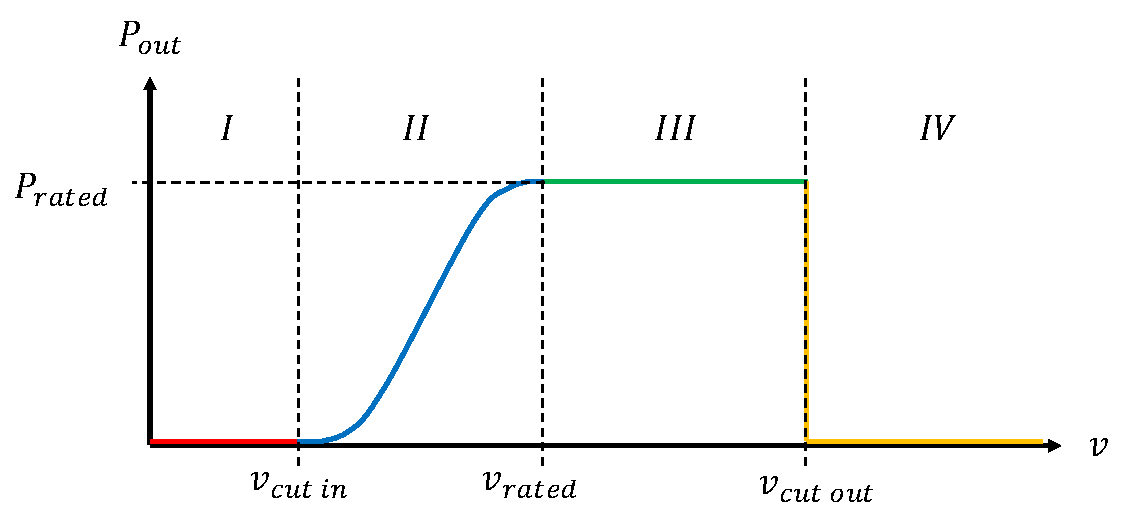
\includegraphics[width = \textwidth]{figures/wind_power_output_profile.pdf}
    \caption{Wind power output profile depending on wind speed, adapted from \cite{windpower}}
    \label{fig:wind_power_profile}
\end{figure}

\subsubsection{Height dependent wind speed}
If we are given the wind speed data $v_1$ at height $h_1$, the wind speed  $v_2$ at the hub height $h_2$ can according to \cite{windspeed} be calculated as:

\setlength{\belowdisplayskip}{12pt} 
\setlength{\abovedisplayskip}{12pt} 

\begin{equation}\label{eq:windspeed at height}
    v_2 = v_1 \frac{\ln{\frac{h_2}{z_0}}}{\ln{\frac{h_1}{z_0}}}
\end{equation}

\noindent where the parameter $z_0$ indicates the roughness length. 

\subsection{Wind Power Constraints}
The set of wind power units is denoted as $\textbf{W}$. The power generated by all units $w \in \textbf{W}$ at time $t$ is expressed as $P^{wind}_{t}$ which is defined as:  

\begin{equation}\label{const:wind}
    0 \leq P^{wind}_{t} \leq \sum_{w \in \textbf{W}} w \cdot P^\text{max}_w
\end{equation}

\noindent where $P^\text{max}_w$ is the maximal possible power output of one wind turbine $w$, calculated with the wind speed according to the equations in Chapter~\ref{chap:wind_basic_formulas}. The limit of the power output $P^{wind}_{t}$ is therefore the power output per wind turbine $P^\text{max}_w$ multiplied by the number of turbines $w$.

\section{Power Balance}
For all times $t$ the supply and demand must be equal. This is expressed through: 

\begin{equation}\label{const:power balance}
    P^{load}_{t} = P_{r, t} + P_{d, t} + P^{dis}_{p,t} - P^{cha}_{p,t} + P^{imp}_{t} - P^{exp}_{t} + P^{solar}_{t} + P^{wind}_{t}
\end{equation}

\section{Renewable Target}
The amount of solar energy $E^{solar}$ and wind energy $E^{wind}$ produced over the time horizon of interest has to fulfill the renewable target depending on the total amount of consumed energy $E^{load}$. 

\begin{equation}\label{const:renewable}
    E^{solar} + E^{wind} = T \cdot E^{load}
\end{equation}

\noindent where $T \in [0..1]$ is the share of the renewables solar and wind. 

\section{Optimization Problem}
Finally, the goal is to minimize the curtailment of solar $Curt^{solar}$, the curtailment of wind $Curt^{wind}$ and the cost for the exchange $C^{Ex}$. The curtailment is defined as the possible power output subtracted by the actual power output and can be defined as: 

\begin{equation}\label{const:curt solar}
    Curt^{solar} = \frac{R}{R^\text{ideal}} \cdot C_s - P^{solar}_{t}
\end{equation}

\begin{equation}\label{const:curt wind}
    Curt^{wind} = \sum_{w \in \textbf{W}} w \cdot P^\text{max}_w -  P^{wind}_{t}
\end{equation}

The weighting factors $W_1, W_2$ and $W_3$ are introduced, due to the lack of investment costs. The curtailment is given in Wh while the cost of the exchange is given in CHF. Therefore the individual elements of the objective function can not be compoared and they do not scale the same way. With the weighting factors the importance of each element can be controlled. 
Therefore, the optimization problem can be formulated as: 

\begin{equation}\label{objective function}
 \begin{array}{l}
    \text{min} \,\, W_1 \cdot Curt^{solar} + W_2 \cdot Curt^{wind} + W_3 \cdot C^{Ex} \\ \\
    \text{s.t. to Constraints \eqref{const:ror power output}-\eqref{const:cost},\eqref{const:solar} and \eqref{const:wind}-\eqref{const:curt wind}}
 \end{array}
\end{equation}